\documentclass{article}
\usepackage{graphicx} % Required for inserting images
\usepackage{geometry}
\usepackage{lipsum}
\usepackage[utf8]{inputenc}
\usepackage{tikz, pgfplots}
\usepackage{afterpage}
\usetikzlibrary{positioning}
\newgeometry{
top = 0.75in,
bottom = 0.75in,
outer = 0.75in,
inner = 1.5in,
}

\title{On the Tisserand's Parameter}
\author{Sreekrishna}
\date{April 2024}

\begin{document}

\maketitle

\section{Introduction}
Tisserand's parameter is essentially used to calculate the degree of perturbation experienced by a larger body which it passes by. The application of the Tisserand's parameter lies in the assessment of Jovian orbits as Jupiter is the primary source for perturbation in most small-body orbits. This is why the parameter is often calculated with respect to the semi-major axis of Jupiter where $a_{planet}$ is considered to be unity. The general equation for Tisserand's parameter is as follows : 
\begin{equation}
    T = \frac{a_{planet}}{a} \ + 2\sqrt{\frac{a}{a_{planet}}(1-e^2)}\ cos\ i
\end{equation}
Taking $a_{planet}$ as unity : 
\begin{equation}
    T_J = \frac{1}{a} \ + 2\sqrt{a(1-e^2)}\ cos\ i
\end{equation}
\\ We use the Tisserand's parameter for its constancy compared to values like $a, e, i$ as outlined very well in \cite{1995EM&P...68...71C} 
\\ This now allows us to apply a criteria to distinguish between the amount of perturbation caused on a small-body with reference to Jupiter. Jovian asteroids can be distinguished from Jovian comets by employing the criterion. \\
Bodies with $T_J >3$ are generally asteroids, whereas bodies with $2<T_J<3 $ are generally Jovian comets. Comets with $T_J <2$ are considered Halley-types.
\section{On the Tisserand parameter}
\subsection{Conservation of the Tisserand's parameter}
\subsubsection{During encounter}
During encounter, other orbital parameters generally change dramatically. This is primarily because of the independence of large single-encounter perturbations from fluctuating interference from the secondary body(in this case, Jupiter). The general equation for the Tisserand's parameter is : 
\begin{equation}
    T_X = \frac{1}{a} + 2\sqrt{\frac{1}{a^2}a(1-e^2)}\ cos\ i_X
\end{equation}
\\ This, although does not ensure the constancy or the conservation of the Tisserand parameter as it undergoes 2 other variations : 
\begin{enumerate}
    \item Orbit is elliptical but equation (3) is only applicable for circular, restricted body
    \item The heliocentric trajectory and the sphere of action of Jupiter(in this case) are not negligible to the heliocentric distance.
\end{enumerate}
 \newpage     
   Now because of the given reasons, $U_X$, the encounter velocity shows a dependence on the true anomaly. To avoid this, we implement the first-order correction prescribed by Tisserand : 

   \begin{equation}
       T'_X = \frac{1}{a} + 2 \frac{\sqrt{a_X p}\ cos\ i_X}{{r_0}^2}
   \end{equation}
\subsubsection{Post-encounter and resonant returns}


\hspace{10cm}
\subsection{The three-body problem and the Jacobi Integral}
The Tisserand parameter is closely related to the Jacobi Integral of the three-body circular orbit problem, which is proven to be a good approximation for the analysis of elliptical orbits by \cite{10.1093/mnras/123.1.1}. The circular three-body problem involves a small body possessing an orbit with respect to two other large bodies. Here, the small body does not show any perturbation towards the other two bodies due to its negligible mass, thus minimising its gravitational effect on its counterparts. The coordinates used in the three-body system are $(\xi, \eta, \zeta)$ in an inertial reference frame. 
Here, we introduce the Jacobi as the only quantity which remains conserved during the encounter of the small body with the secondary body(in this case, Jupiter). This is proven by taking a function $I$ \footnote{$\rho_1$ and $\rho_2$ here are the distances between the axes and the objects}: 
\begin{equation}
    I = 2 \bigg( \frac{Gm_1}{\rho_1}+ \frac{Gm_2}{\rho_2}\bigg) + 2\omega(\xi \dot{\eta}-\eta \dot{\xi})-\dot{\xi^2}-\dot{\eta^2}-\zeta^2
\end{equation}
The time derivative of $I$ can then be shown, through algebraic manipulations, to be constant. This function, $I$, is called the Jacobi Integral and is conserved during the interaction. For the calculation of the Tisserand Parameter, Jacobi integral can only be employed for making short-term predictions. This is due to the elliptical orbit of Jovian orbits, whereas the evaluation of the Jacobi is implemented on three-body circular systems.



\section{Use of the Tisserand Criteria}
Generally, in taxonomy schemes, like \cite{1996ASPC..107..173L}, which make use of the Tisserand's Parameter to categorize comets and asteroids, comets with $T_J < 2$ are considered nearly-isotropic, meaning their inclination range has a fairly uniform distribution. Comets with $T_J > 2$ are called ecliptic as their inclination distribution comes out to be respectably flat. The parent categorisation of comets, prior to the recommendations laid in \cite{1996ASPC..107..173L} was on the basis of the temporal dynamics of their orbits. Wherein, the periods and other orbital elements of its' orbits were taken into account to draw up the categorisation parameter; here, orbits with periods greater than $200$ years were called long-period comets and ones with periods lesser than $200$ years were called short-period comets. This was abandoned because of the lack of accuracy in the observation of long-period orbits where it became difficult to establish, without a high threshold of uncertainty, if the comet that was passing was observed historically at the same orbital elements. This is why new criteria schemes incorporate a more consistent parent parameter, that is the Tisserand's. 
\subsection{Parameters of the criteria}
As previously mentioned, comets with $T_J>2$ are called ecliptic; but this metric is not enough to usefully narrow down the classification. So, under ecliptic-type comets, we further categorise it on the basis of its $T_J$ and its semi-major axis with respect to that of Jupiter. Here, comets with $T_J>3$ and $a<a_J$ are considered to be of Encke-type; these comets generally have their orbits completely in the interior of Jupiter. Comets with $2<T_J<3$ are considered to be in the Jupiter-family and their orbits are determined completely by Jupiter's perturbation effects on it. Lastly, comets with $T_J>3$ and $a>a_J$ lie completely in the exterior of the Jovian orbit and are distinguished as the Chiron family of comets. 
Now for orbits with $T_J<2$, which are termed nearly-isotropic are further classified into two on the basis of their semi-major axis :
\begin{enumerate}
    \item Comets with $a>10000$AU are called New comets and are subject to a considerable amount of research
    \item Comets with $a<10000$AU are called returning comets and due to the large size of the family, are further classified : 
        \begin{enumerate}
            \item External - These have comets which possess orbits with $a>40$AU
            \item Halley-type - These have comets which possess orbits with $a<40$AU
        \end{enumerate}
            
\end{enumerate}



Objects with $T_J$ very close to, but less than $3$ often have slow encounters with Jupiter, causing larger perturbations to their orbital elements post-encounter. Objects with $T_J$ larger than $3$ are not afflicted by Jupiter's gravitational(at least in the approximated circular three-body case) as their orbits are found completely exterior or completely interior to the orbit of Jupiter, disabling them completely from crossing Jupiter. 
\\ 
\\
\begin{figure}[htbp]
    \centering
    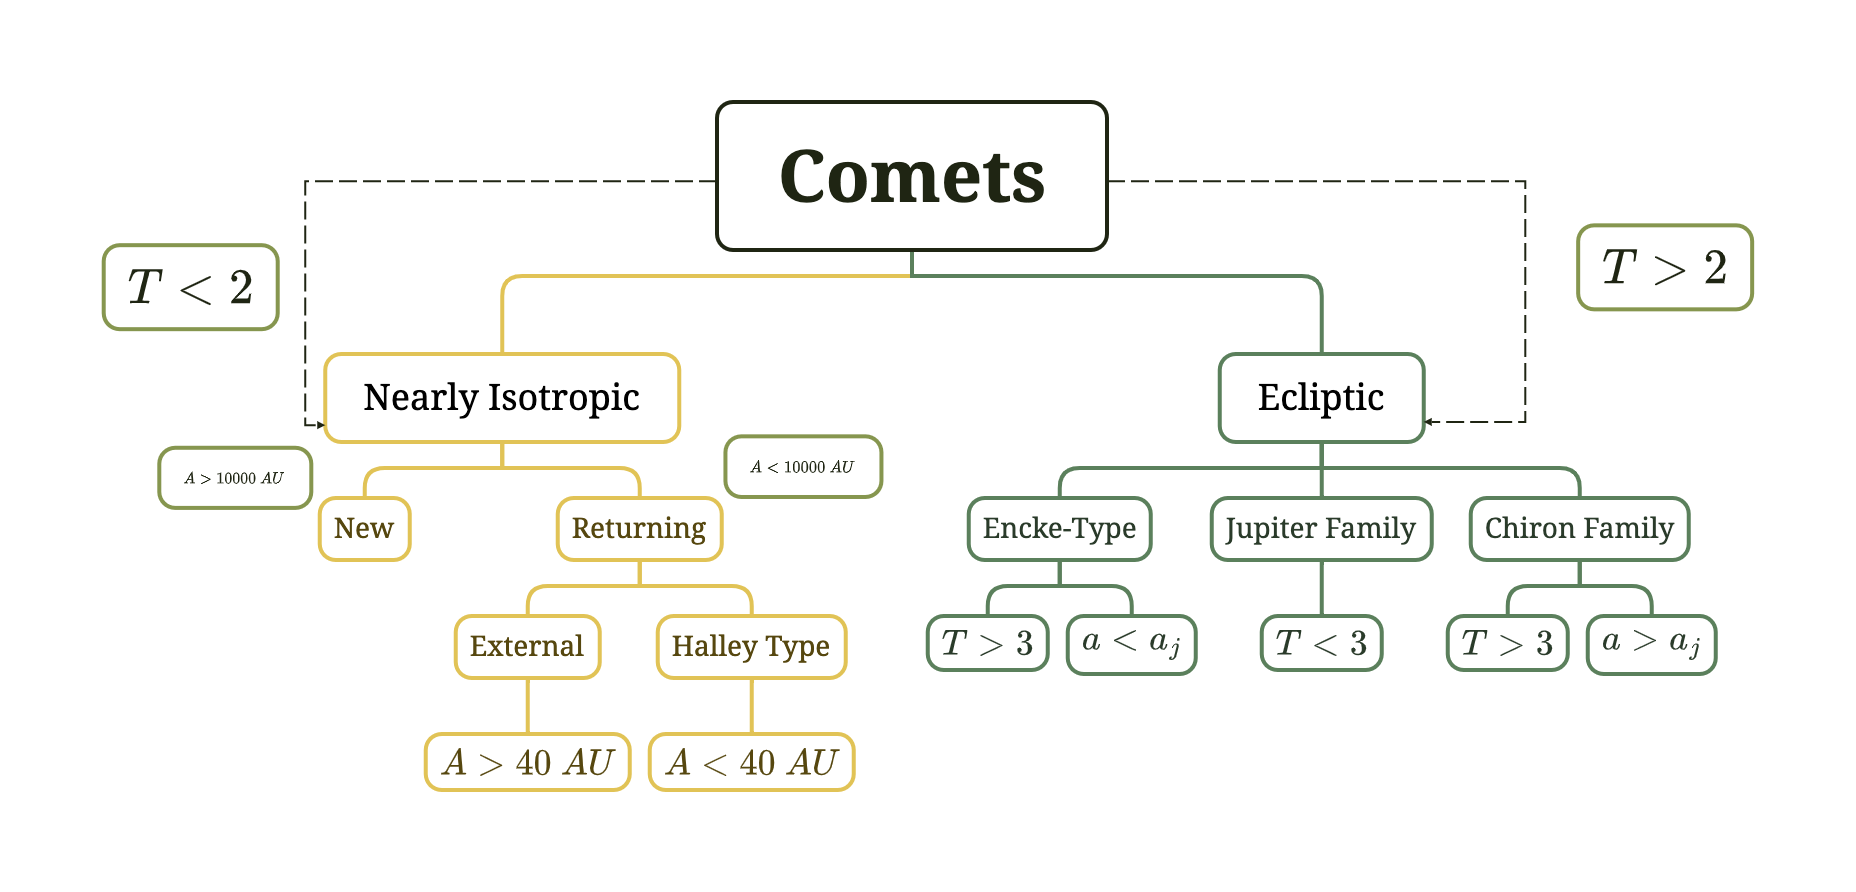
\includegraphics[width=8cm]{Image/Comets.png}
    \caption{Classification of comets on the basis of $T_J$}
    \label{fig:enter-label}
\end{figure}


\section{Analysis of various comets and asteroids}

\subsection{109P/Swift-Tutle}
The thorough analysis of the Swift-Tutle is done in \cite{article} 
\begin{figure}[htbp]
    \centering
    \includegraphics[width=8cm]{Image/Tisserand_Figures/Swift-Tutle.png}
    \caption{Orbit of Swift-Tutle}
    \label{fig:enter-label}
\end{figure}
\newpage
\subsection{Lovejoy}
\begin{figure}[htbp]
    \centering
    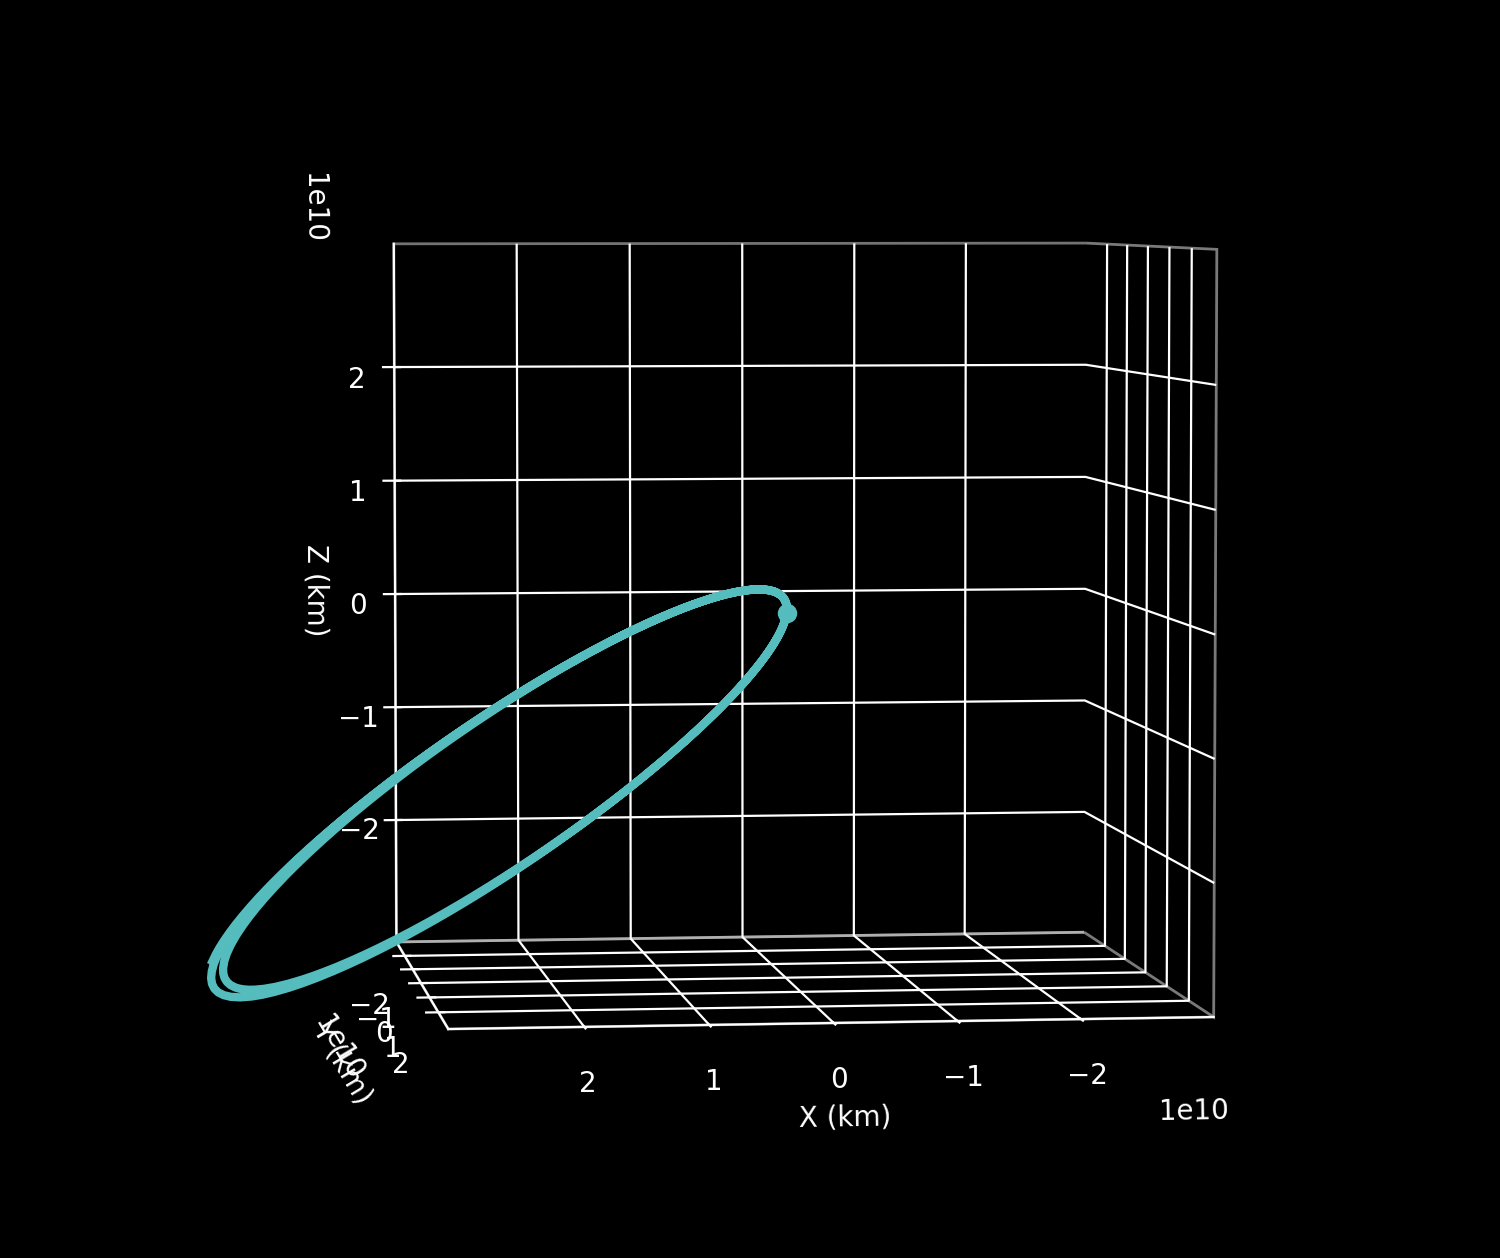
\includegraphics[width=8cm]{Image/Tisserand_Figures/Lovejoy-Comet Integrated.png}
    \caption{Orbit of Lovejoy}
    \label{fig:enter-label}
\end{figure}
\subsection{2P/Encke}
\begin{figure}[htbp]
    \centering
    \includegraphics[width=8cm]{Image/Tisserand_Figures/Screenshot 2024-04-10 at 7.37.22 AM.png}
    \caption{Orbit of 2P/Encke}
    \label{fig:enter-label}
\end{figure}
\newpage
\subsection{3200 Phaethon}
3200 Phaethon
\begin{figure}[htbp]
    \centering
    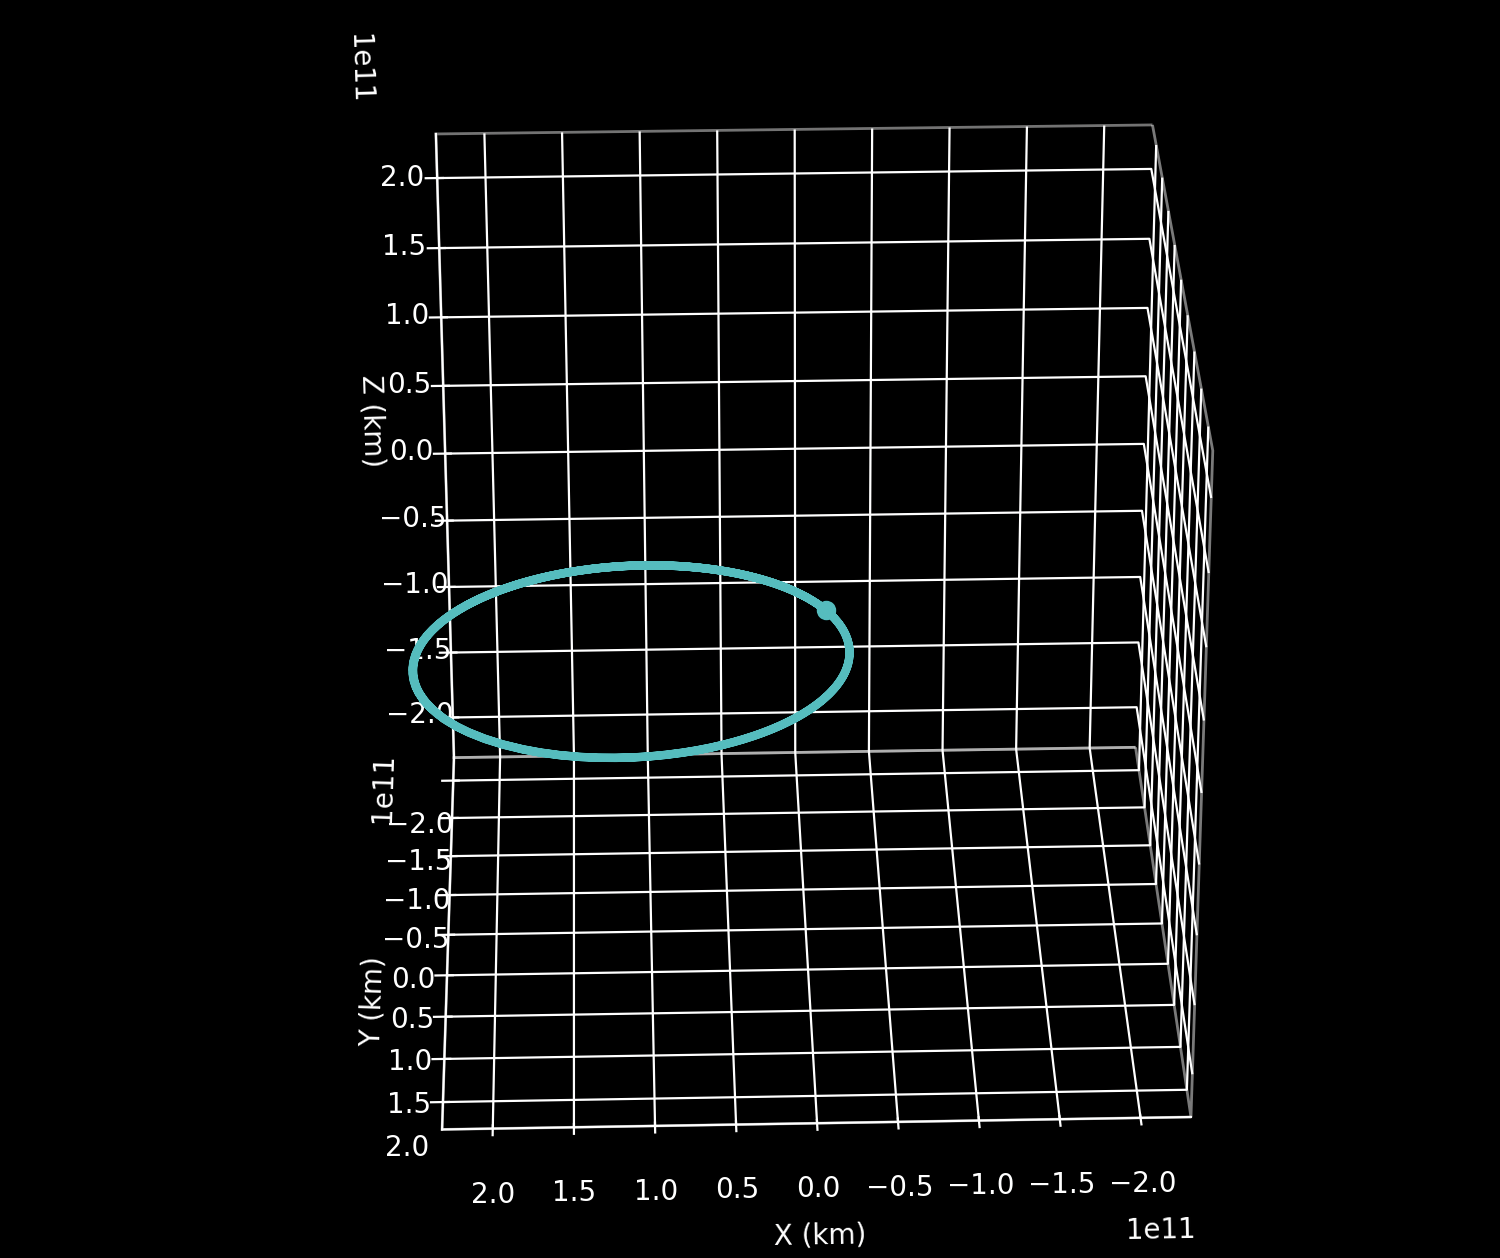
\includegraphics[width=8cm]{Image/Tisserand_Figures/3200Phaethon.png}
    \caption{Orbit of 3200/Phaethon}
    \label{fig:enter-label}
\end{figure}
\subsection{Ceres}
\begin{figure}[htbp]
    \centering
    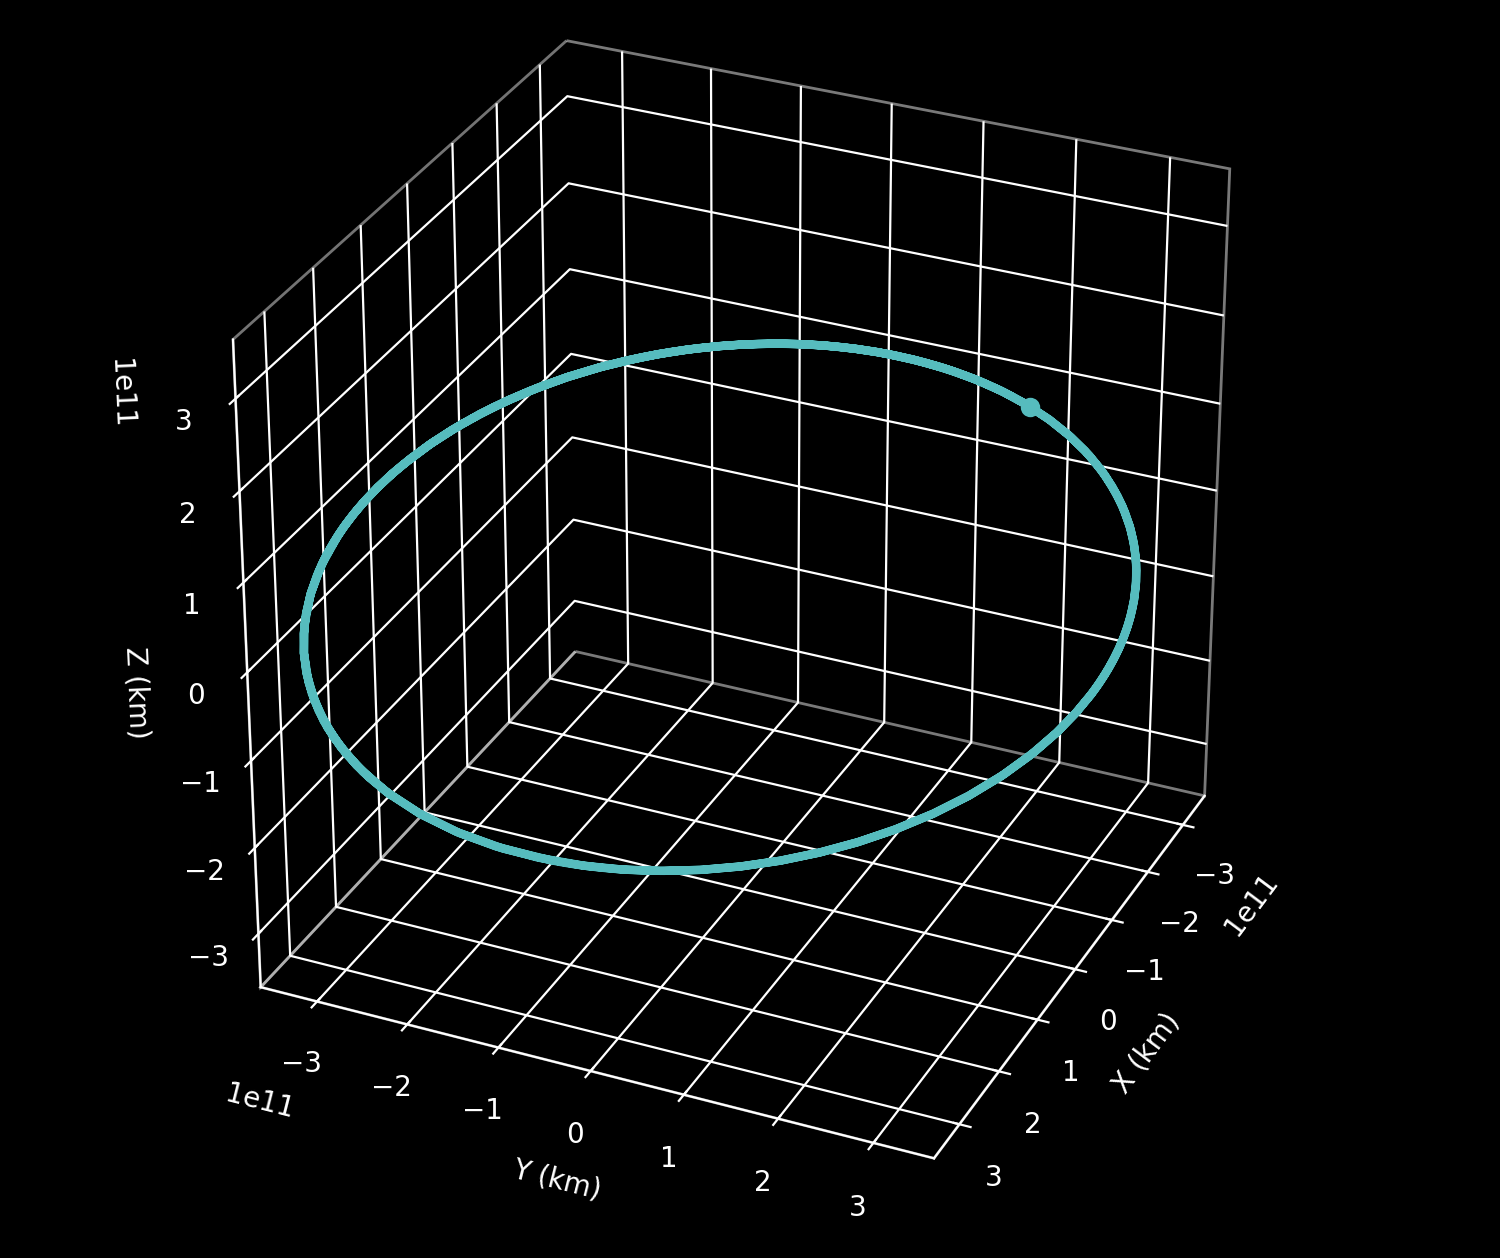
\includegraphics[width=8cm]{Image/Tisserand_Figures/Ceres.png}
    \caption{Orbit of Ceres}
    \label{fig:enter-label}
\end{figure}
\newpage
\subsection{Apophis}
\begin{figure}[htbp]
    \centering
    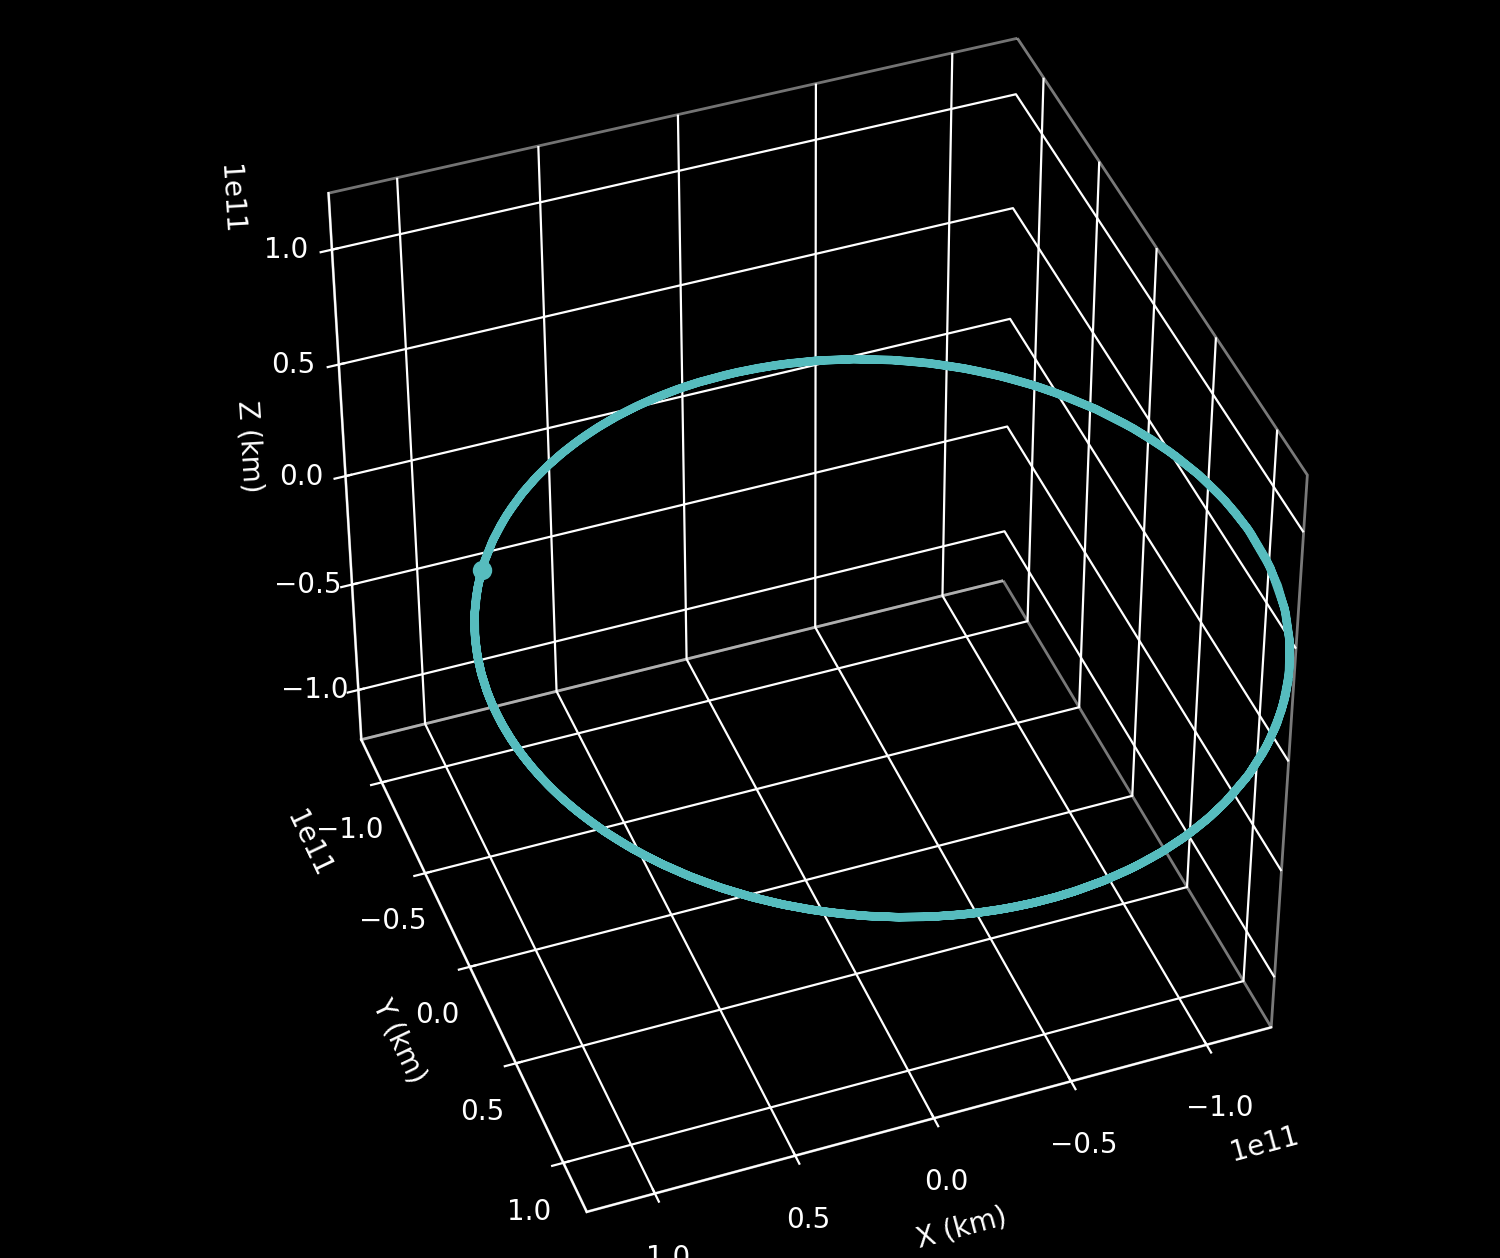
\includegraphics[width=8cm]{Image/Tisserand_Figures/Apophis.png}
    \caption{Orbit of Apophis}
    \label{fig:enter-label}
\end{figure}
\subsection{Pluto}
\begin{figure}[htbp]
    \centering
    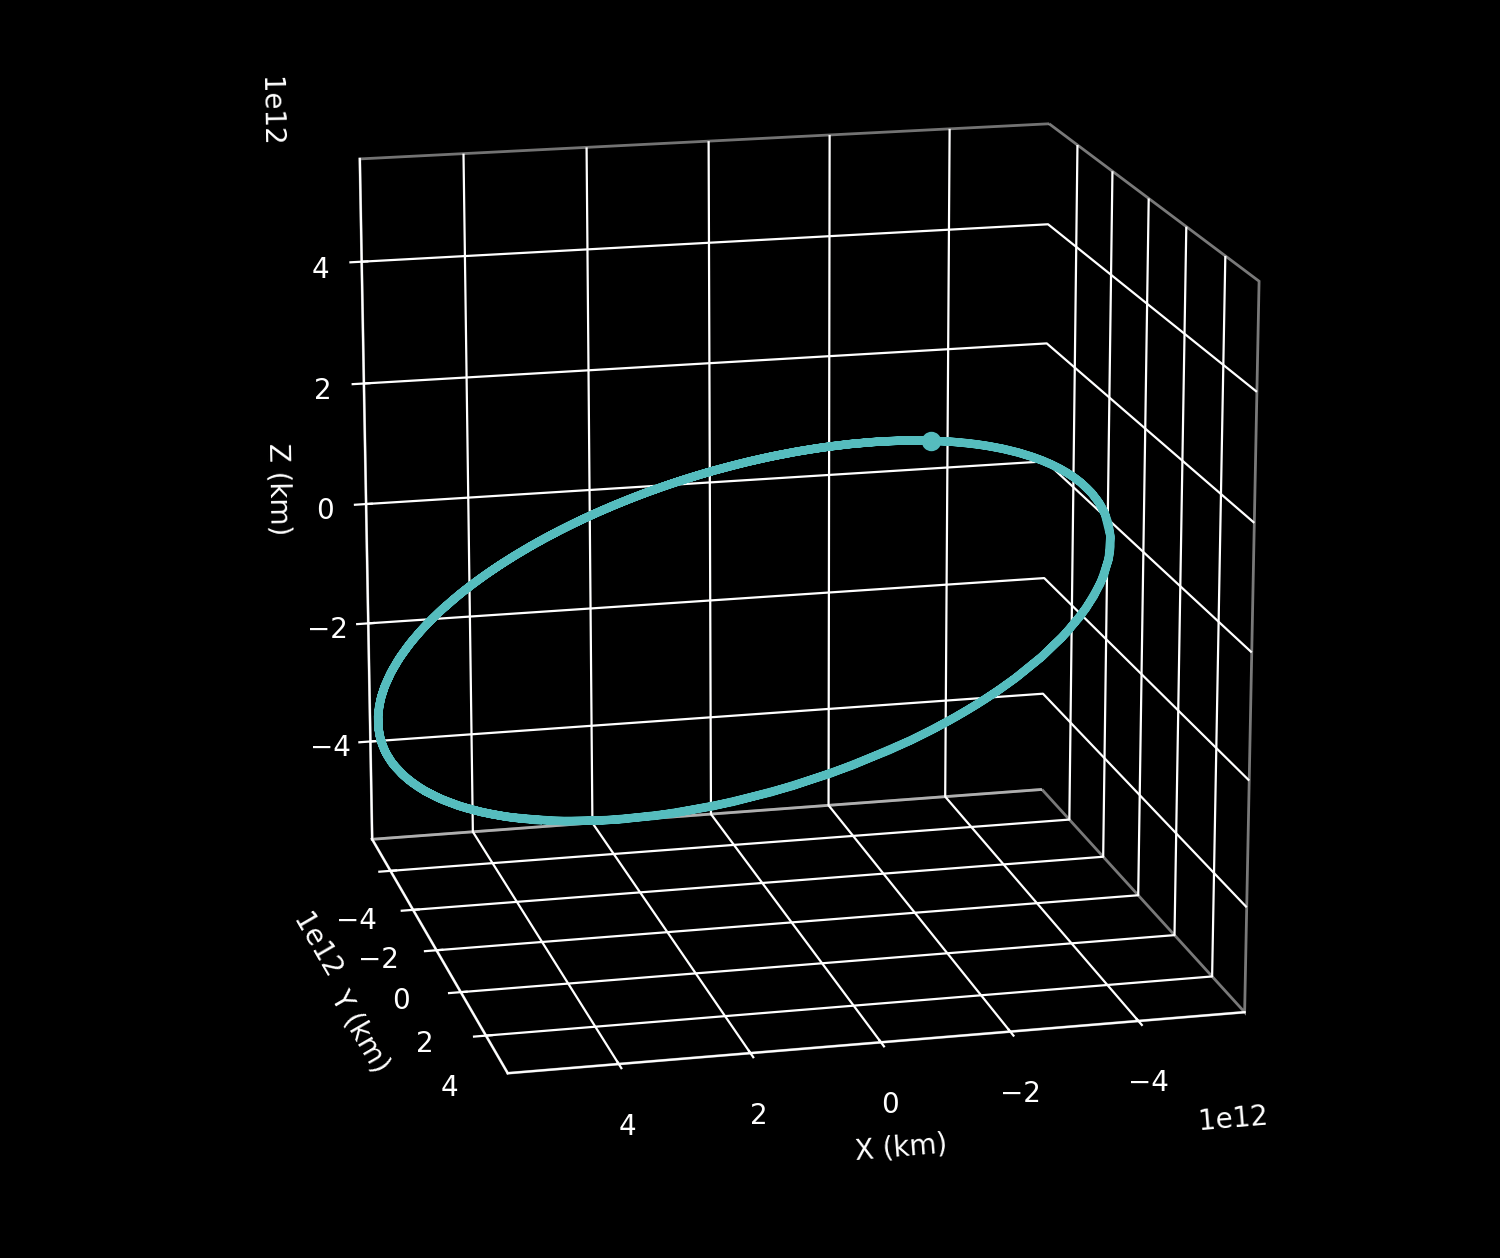
\includegraphics[width=8cm]{Image/Tisserand_Figures/Pluto.png}
    \caption{Orbit of Pluto}
    \label{fig:enter-label}
\end{figure}
\newpage
\subsection{Shoemaker-Levy 9}
\begin{figure}[htbp]
    \centering
    \includegraphics[width=8cm]{Image/Tisserand_Figures/Shoemaker-Levy9.png}
    \caption{Orbit of Shoemaker-Levy 9}
    \label{fig:enter-label}
\end{figure}

\newpage
\bibliographystyle{plain}
\bibliography{references}
\end{document}
 